\begin{SCn}

\scnsectionheader{\currentname}

\scnstartsubstruct

\scnheader{Предметная область темпоральных сущностей}
\scnidtf{Предметная область темпоральных связей и отношений}
\scnidtf{Предметная область временных сущностей}
\scniselement{предметная область}
\scnsdmainclasssingle{временная сущность}
\scnsdclass{прошлая сущность;настоящая сущность;будущая сущность;временная связь;ситуация;процесс;процесс в sc-памяти;процесс во внешней среде ostis-системы;материальная сущность;воздействие;отношение;класс временных связей;класс временных и постоянных связей;множество;ситуативное множество;неситуативное множество;частично ситуативное множество;темпоральная связь;темпоральное отношение;начало;завершение;длительность;тысячелетие;век;год;месяц;сутки;час;минута;секунда}
\scnsdrelation{воздействующая сущность*;объект воздействия*;начальная ситуация*;причинная ситуация*;конечная ситуация*;событие*;последний добавленный sc-элемент\scnrolesign;темпоральное включение*;темпоральная часть*;начальный этап*;конечный этап*;промежуточный этап*;темпоральное включение без совпадения начальных и конечных моментов*;темпоральное включение с совпадением начальных моментов*;темпоральное включение с совпадением конечных моментов*;темпоральное совпадение*;темпоральное объединение*;темпоральная декомпозиция*;темпоральная смежность*;темпоральная последовательность с промежутком*;темпоральная последовательность с пересечением*;номер тысячелетия\scnrolesign;номер века\scnrolesign;номер года\scnrolesign;номер месяца в году\scnrolesign;номер суток в месяце\scnrolesign;номер часа в дне\scnrolesign;номер минуты в часе\scnrolesign;номер секунды в минуте\scnrolesign}

\scnheader{временная сущность}
\scnidtf{временно существующая сущность}
\scnidtf{нестационарная сущность}
\scnidtf{сущность, имеющая и/или начало, и/или конец своего существования}
\scnidtf{sc-элемент, являющийся знаком некоторой временно существующей сущности}
\scnidtf{сущность, обладающая темпоральными характеристиками (длительностью, начальным моментом, конечным моментом и т.д.)}
\scnreltoset{разбиение}{прошлая сущность;настоящая сущность;будущая сущность}
\scnreltoset{разбиение}{временная связь;ситуация;процесс;материальная сущность}
\scnexplanation{Следует отличать:
\begin{scnitemize}
    \item временный характер сущности, обозначаемой \textit{sc-элементом};
    \item временный характер существования самого \textit{sc-элемента} в рамках \textit{sc-памяти};
\end{scnitemize}
В ходе обработки информации каждый \textit{sc-элемент} может быть удален из \textit{sc-памяти}.}

\scnheader{прошлая сущность}
\scnidtf{сущность, существовавшая в прошлом времени}
\scnidtf{сущность прошлого времени}
\scnidtf{сущность, завершившая свое существование}

\scnheader{настоящая сущность}
\scnidtf{сущность, существующая в текущий момент времени}
\scnidtf{сущность, существующая сейчас}
\scnidtf{сущность настоящего времени}

\scnheader{будущая сущность}
\scnidtf{возможно будущая сущность}
\scnidtf{прогнозируемая временная сущность}
\scnidtf{временная сущность, которая может существовать в будущем}
\scnidtf{сущность, которая может или должна начать свое существование в будущем времени}
\scnrelfrom{включение}{инициированное действие}
\scnexplanation{Каждой \textbf{\textit{будущей сущности}} можно поставить в соответствие вероятность ее возникновения.}

\scnheader{временная связь}
\scnidtf{нестационарная связь}
\scnidtf{временно существующая связь}
\scnexplanation{Каждая \textbf{\textit{временная связь}} представляет собой \textit{связку}, принадлежащую множеству \textit{временных сущностей}.

Понятие \textbf{\textit{временной связи}} не следует путать с понятием \textit{темпоральной связи}, которая сама является \textit{постоянной сущностью}, описывающей то, как связаны во времени некоторые \textit{временные сущности}.
}

\scnheader{ситуация}
\scnidtf{состояние}
\scnidtf{временная структура}
\scnidtf{временно существующая структура}
\scnidtf{квазистационарная структура}
\scnidtf{состояние некоторой динамической системы, описываемое с некоторой степенью детализации (подробности)}
\scnidtf{квазистационарная структура, существующая временно (в течение некоторого отрезка времени)}
\scnrelto{включение}{структура}
\scnexplanation{Под ситуацией понимается \textit{структура}, содержащая, по крайней мере, один элемент, который является \textit{временной сущностью}. Наличие в рамках ситуации нескольких \textit{временных сущностей} говорит о том, что существует момент времени (в прошлом, настоящем или будущем), в который все они существуют одновременно.}

\scnheader{процесс}
\scnidtf{процесс преобразования некоторой временной сущности из одного состояния в другое}
\scnidtf{процесс перехода от одной ситуации к другой}
\scnidtf{переходный процесс}
\scnidtf{абстрактный процесс}
\scnidtf{информационная модель некоторых преобразований}
\scnidtf{динамическая sc-модель}
\scnidtf{динамическая структура}
\scnrelfrom{включение}{воздействие}
\scnrelto{включение}{структура}
\scnexplanation{Каждый \textbf{\textit{процесс}} определяется (задается) либо возникновением или исчезновением связей, связывающих заданную \textit{временную сущность} с другими сущностями, либо возникновением или исчезновением связей, связывающих части указанной \textit{временной сущности} с другими сущностями. 

Многим \textbf{\textit{процессам}} можно поставить в соответствие \textit{ситуацию}, которая является его \textit{начальной ситуацией*} и \textit{ситуацию}, которая является его \textit{конечной ситуацией*}, то есть указать \textit{ситуации}, переход между которыми осуществляется в ходе \textbf{\textit{процесса}}.

При этом знаки тех \textit{временных сущностей}, с которыми связаны изменения, описываемые некоторым \textbf{\textit{процессом}}, входят в данный \textbf{\textit{процесс}} как элементы и при необходимости уточняются дополнительными \textit{ролевыми отношениями}.}
\scnreltoset{разбиение}{процесс в sc-памяти;процесс во внешней среде ostis-системы}

\scnheader{процесс в sc-памяти}

\scnheader{процесс во внешней среде ostis-системы}

\scnheader{материальная сущность}
\scnexplanation{Каждой \textbf{\textit{материальной сущности}} можно поставить в соответствие различные \textit{процессы}, описывающие ее преобразование из одного состояния в другое.}

\scnheader{воздействие}
\scnidtf{процесс, осуществляющийся на основе (в результате) воздействия одной сущности на другую}
\scnrelfrom{включение}{действие}
\scnexplanation{Каждому \textbf{\textit{воздействию}} может быть поставлена в соответствие (1) некоторая \textit{воздействующая сущность*}, т.е. сущность, осуществляющая \textbf{\textit{воздействие}} (в частности, это может быть некоторое физическое поле), и (2) некоторый \textit{объект воздействия*}, т.е. сущность, на которую воздействие направлено. Если \textbf{\textit{воздействие}} связано с \textit{материальной сущностью}, то его объектом воздействия является либо сама эта \textit{материальная сущность}, либо некоторая ее пространственная часть.}

\scnheader{воздействующая сущность*}

\scnheader{объект воздействия*}

\scnheader{начальная ситуация*}
\scnidtf{начальная ситуация процесса*}
\scnidtf{исходная ситуация*}
\scniselement{бинарное отношение}
\scnexplanation{Связки отношения \textbf{\textit{начальная ситуация*}} связывают некоторый \textit{процесс} и некоторую ситуацию, являющуюся начальной для этого \textit{процесса}, и, как правило, изменяемой в течение выполнения этого \textit{процесса}.

Первым компонентом каждой связки отношения \textbf{\textit{начальная ситуация*}} является знак \textit{процесса}, вторым – знак начальной \textit{ситуации}.}

\scnheader{причинная ситуация*}
\scniselement{бинарное отношение}
\scnrelto{включение}{начальная ситуация*}
\scnexplanation{Под причинной ситуацией понимается такая \textit{начальная ситуация*}, которая обладает достаточной полнотой для однозначного задания инициируемого \textit{процесса}.}

\scnheader{конечная ситуация*}
\scnidtf{конечная ситуация процесса*}
\scnidtf{результирующая ситуация*}
\scniselement{бинарное отношение}
\scnexplanation{Связки отношения \textbf{\textit{конечная ситуация*}} связывают некоторый \textit{процесс} и некоторую \textit{ситуацию}, ставшую результатом выполнения этого \textit{процесса}, то есть его следствием.

Первым компонентом каждой связки отношения \textbf{\textit{конечная ситуация*}} является знак \textit{процесса}, вторым – знак конечной \textit{ситуации}.}

\scnheader{событие*}
\scniselement{бинарное отношение}
\scnexplanation{Связки отношения \textbf{\textit{событие*}} связывают знак процесса и ориентированную пару, первым компонентом которой является знак \textit{начальной ситуации*} данного процесса, вторым компонентом – знак \textit{конечной ситуации*} данного процесса.}
\scnrelfrom{типичная семантическая окрестность}{
\scnfilescg{figures/sd_temp_entities/event.png}
}

\scnheader{отношение}
\scnreltoset{разбиение}{класс временных связей;класс постоянных связей;класс временных и постоянных связей}

\scnheader{класс временных связей}
\scnidtf{отношение, все связки которого являются нестационарными}
\scnexplanation{В общем случае \textbf{\textit{класс временных связей}} не является \textit{ситуативным множеством}, поскольку факт принадлежности некоторой \textit{временной связи} такому классу следует считать постоянным, а не временным, поскольку временность/постоянство связи и ее семантический тип, задаваемый классом (отношением), это принципиально разные параметры (характеристики, признаки) любой связи.}

\scnheader{класс постоянных связей}
\scnidtf{отношение, все связки которого являются стационарными}

\scnheader{класс временных и постоянных связей}
\scnidtf{отношение, некоторые (но не все) связки которого являются нестационарными}

\scnheader{множество}
\scnreltoset{разбиение}{ситуативное множество;неситуативное множество;частично ситуативное множество}

\scnheader{ситуативное множество}
\scnidtf{полностью ситуативное множество}
\scnexplanation{Под \textbf{\textit{ситуативным множеством}} понимается постоянное множество, у которого все выходящие из него связи принадлежности являются \textit{временными сущностями}.

В частности, ситуативное множество может использоваться как вспомогательная динамическая структура, которая содержит элементы некоторых структур, обрабатываемые в данный момент, например, это может быть копия некоторого множества, из которой постепенно удаляются элементы по мере их просмотра и обработки. В случае, когда такая структура содержит всего один элемент, ее можно считать \underline{указателем} на данный элемент, при этом в разные моменты времени это могут быть разные элементы.}

\scnheader{последний добавленный sc-элемент’}
\scniselement{ролевое отношение}

\scnheader{неситуативное множество}
\scnexplanation{Под \textbf{\textit{неситуативным множеством}} понимается постоянное множество, у которого все выходящие из него связи принадлежности являются \textit{постоянными сущностями}.}

\scnheader{частично ситуативное множество}
\scnexplanation{Под \textbf{\textit{частично ситуативным множеством}} понимается постоянное множество, у которого некоторые (но не все) выходящие из него связи принадлежности являются \textit{временными сущностями}.}

\scnheader{темпоральная связь}
\scnidtf{постоянная связь, описывающая связь во времени между временными сущностями}

\scnheader{темпоральное отношение}
\scnrelto{семейство подмножеств}{темпоральная связь}
\scnidtf{класс темпоральных связей}
\scnidtf{отношение, задающее темпоральные связи между временными сущностями}
\scnhaselement{темпоральное включение*}
\scnhaselement{темпоральное объединение*}
\scnhaselement{темпоральная декомпозиция*}
\scnhaselement{темпоральная смежность*}
\scnhaselement{темпоральная последовательность с промежутком*}
\scnhaselement{темпоральная последовательность с пересечением*}

\scnheader{темпоральное включение*}
\scnexplanation{Связки отношения \textbf{\textit{темпоральное включение*}} связывают две \textit{временные сущности}, период существования одной из которых полностью включается в период существования второй.\\
Первым компонентом каждой связки отношения \textbf{\textit{темпоральное включение*}} является знак \textit{временной сущности}, \textit{длительность} существования которой больше.}
\scnrelfromlist{включение}{темпоральная часть*;темпоральное включение без совпадения начальных и конечных моментов*;темпоральное совпадение*;темпоральное включение с совпадением начальных моментов*;темпоральное включение с совпадением конечных моментов*}

\scnheader{темпоральная часть*}
\scnidtf{этап (период) заданной временной сущности*}
\scnidtf{этап процесса существования временной сущности*}
\scnrelfromlist{включение}{начальный этап*;конечный этап*;промежуточный этап*}
\scnrelfrom{типичная семантическая окрестность}{
\scnfilescg{figures/sd_temp_entities/temporal_part.png}
}
\scnrelfrom{иллюстрация}{
\scnfileimage{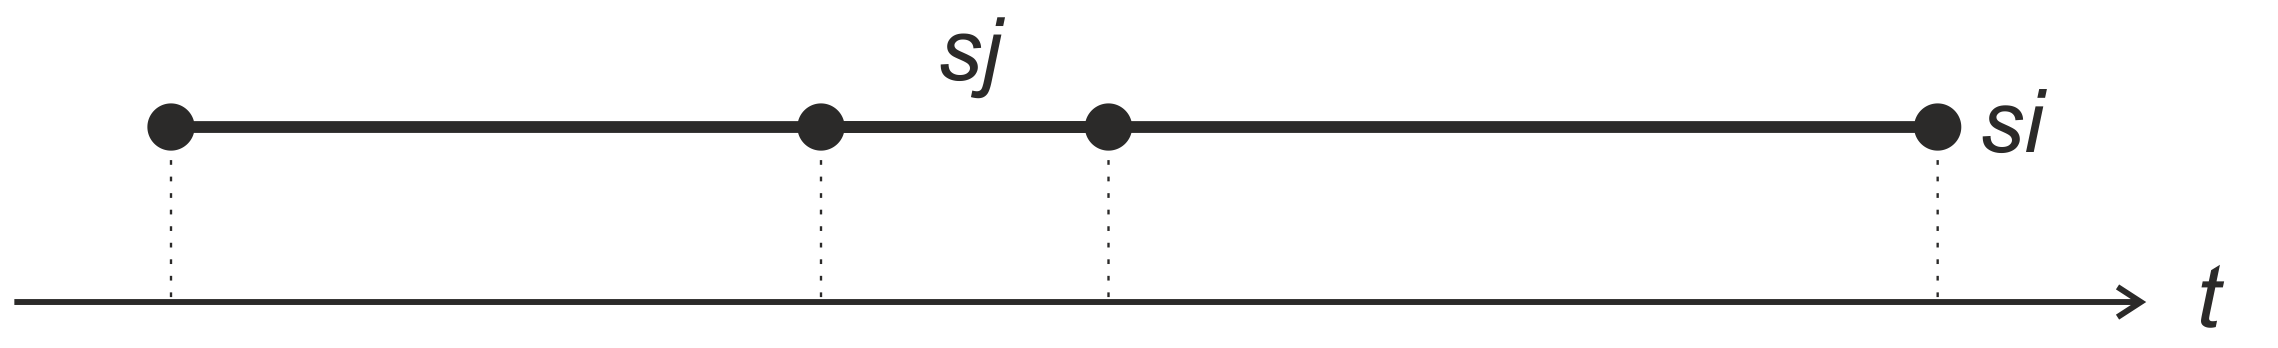
\includegraphics[width=1\linewidth]{figures/sd_temp_entities/img_temporal_part.png}}}
\scntext{примечание}{Связки отношения \textbf{\textit{темпоральная часть*}} связывают две \textit{временные сущности}, одна из которых является частью другой, например, действие и одно из его поддействий. Соответственно, период существования одной из этих сущностей всегда будет включаться в период существования другой (большей).

В отличие от более общего отношения \textit{темпоральное включение*}, связки которого могут связывать любые \textit{временные сущности}, связки отношения \textbf{\textit{темпоральное включение*}} связывают только \textit{временные сущности}, одна из которых является частью другой.}

\scnheader{начальный этап*}

\scnheader{конечный этап*}

\scnheader{промежуточный этап*}

\scnheader{темпоральное включение без совпадения начальных и конечных моментов*}
\scnidtf{строгое темпоральное включение*}
\scnrelfrom{типичная семантическая окрестность}{
\scnfilescg{figures/sd_temp_entities/strict_temporal_inclusion.png}}
\scnrelfrom{иллюстрация}{
\scnfileimage{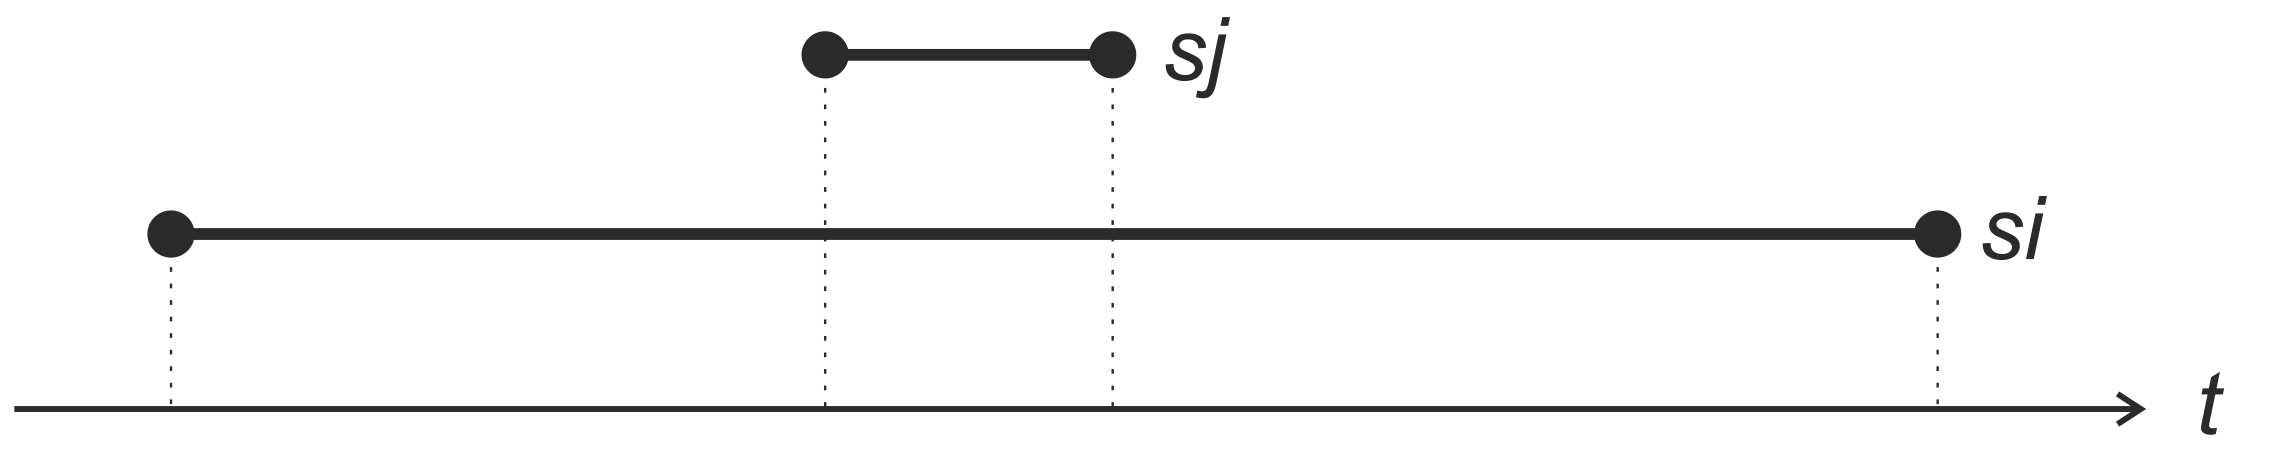
\includegraphics[width=1\linewidth]{figures/sd_temp_entities/img_strict_temporal_inclusion.png}}}
%
% темпоральное включение без совпадения начальных и конечных %моментов
%

\scnheader{темпоральное включение с совпадением начальных моментов*}
\scnrelfrom{типичная семантическая окрестность}{
\scnfilescg{figures/sd_temp_entities/temporal_include_with_match_start_points.png}}
\scnrelfrom{иллюстрация}{
\scnfileimage{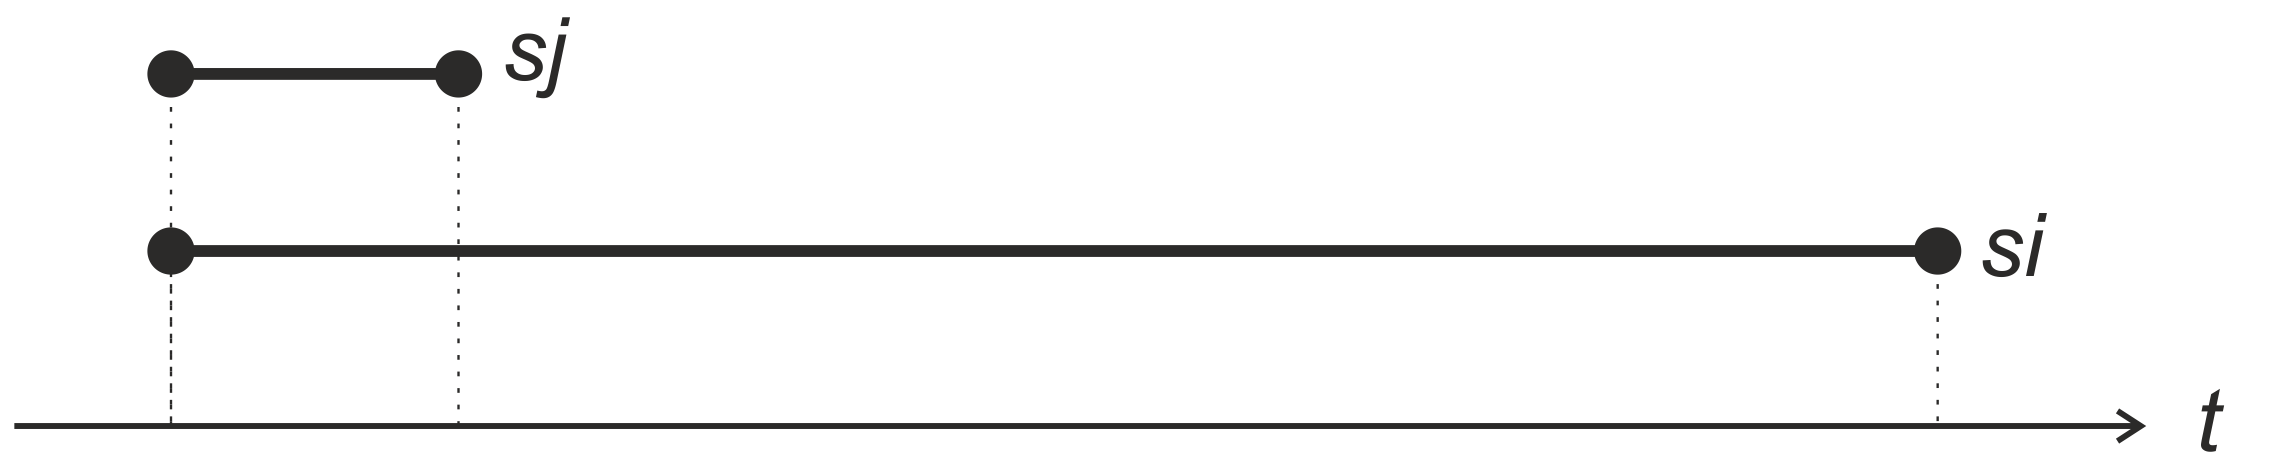
\includegraphics[width=1\linewidth]{figures/sd_temp_entities/img_temporal_include_with_match_start_points.png}}}

\scnheader{темпоральное включение с совпадением конечных моментов*}
\scnrelfrom{типичная семантическая окрестность}{
\scnfilescg{figures/sd_temp_entities/temporal_include_with_terminal_point_match.png}}
\scnrelfrom{иллюстрация}{
\scnfileimage{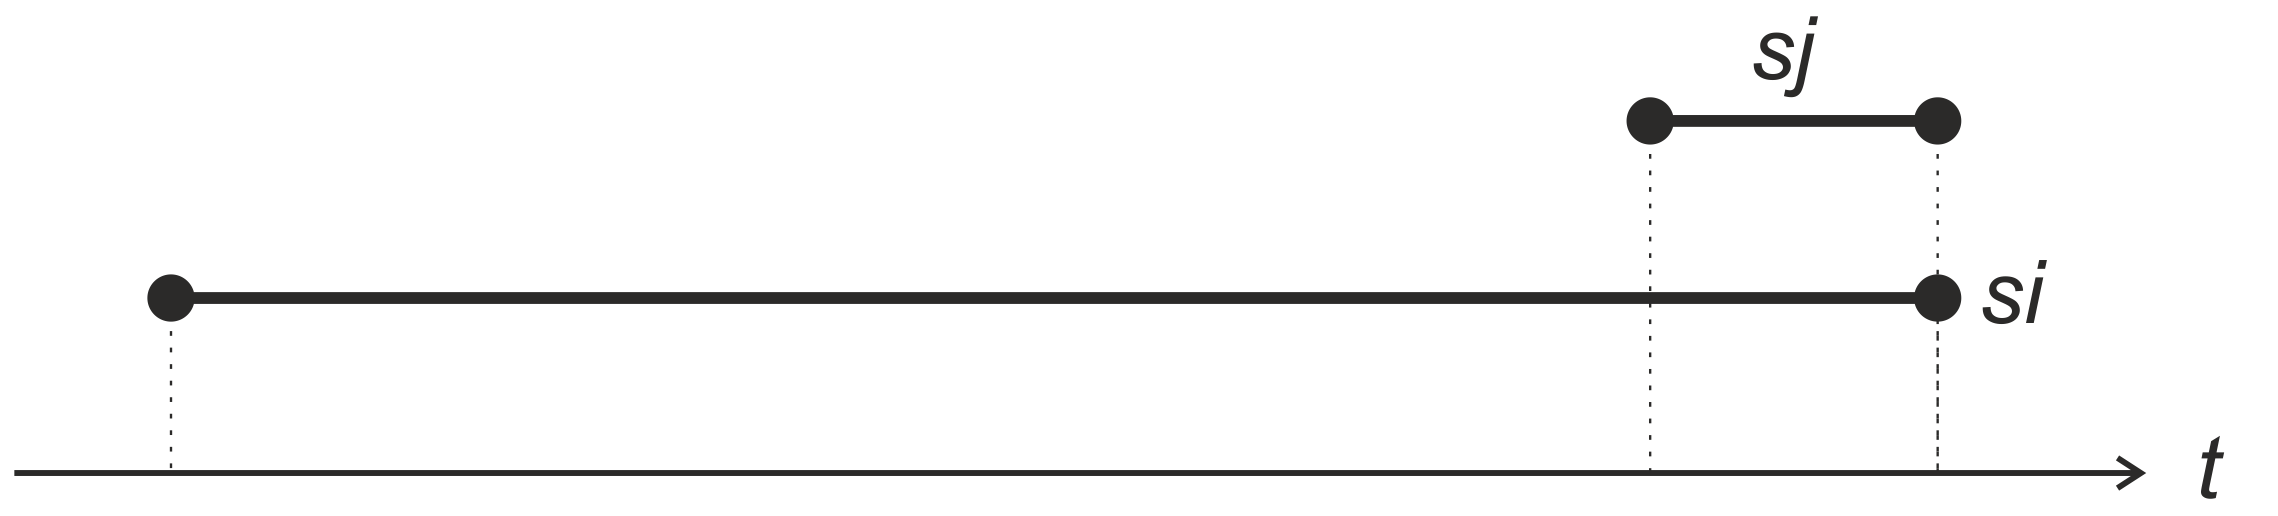
\includegraphics[width=1\linewidth]{figures/sd_temp_entities/img_temporal_include_with_terminal_point_match.png}}}

\scnheader{темпоральное совпадение*}
\scnidtf{совпадение начала и завершения*}

\scnheader{темпоральное объединение*}
\scnrelfrom{типичная семантическая окрестность}{
\scnfilescg{figures/sd_temp_entities/temporal_union.png}}
\scnrelfrom{иллюстрация}{
\scnfileimage{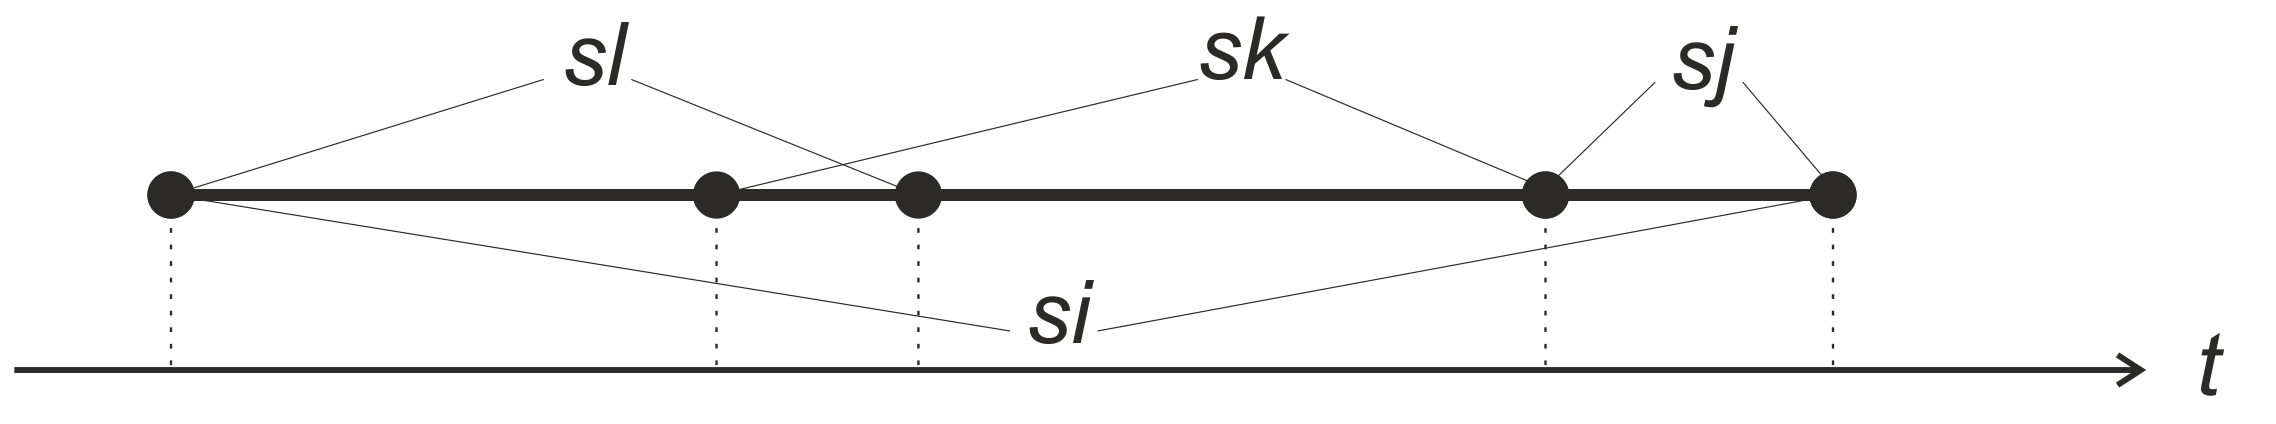
\includegraphics[width=1\linewidth]{figures/sd_temp_entities/img_temporal_union.png}}}

\scnheader{темпоральная декомпозиция*}
\scnrelfrom{типичная семантическая окрестность}{
\scnfilescg{figures/sd_temp_entities/temporal_decomposition.png}}
\scnrelfrom{иллюстрация}{
\scnfileimage{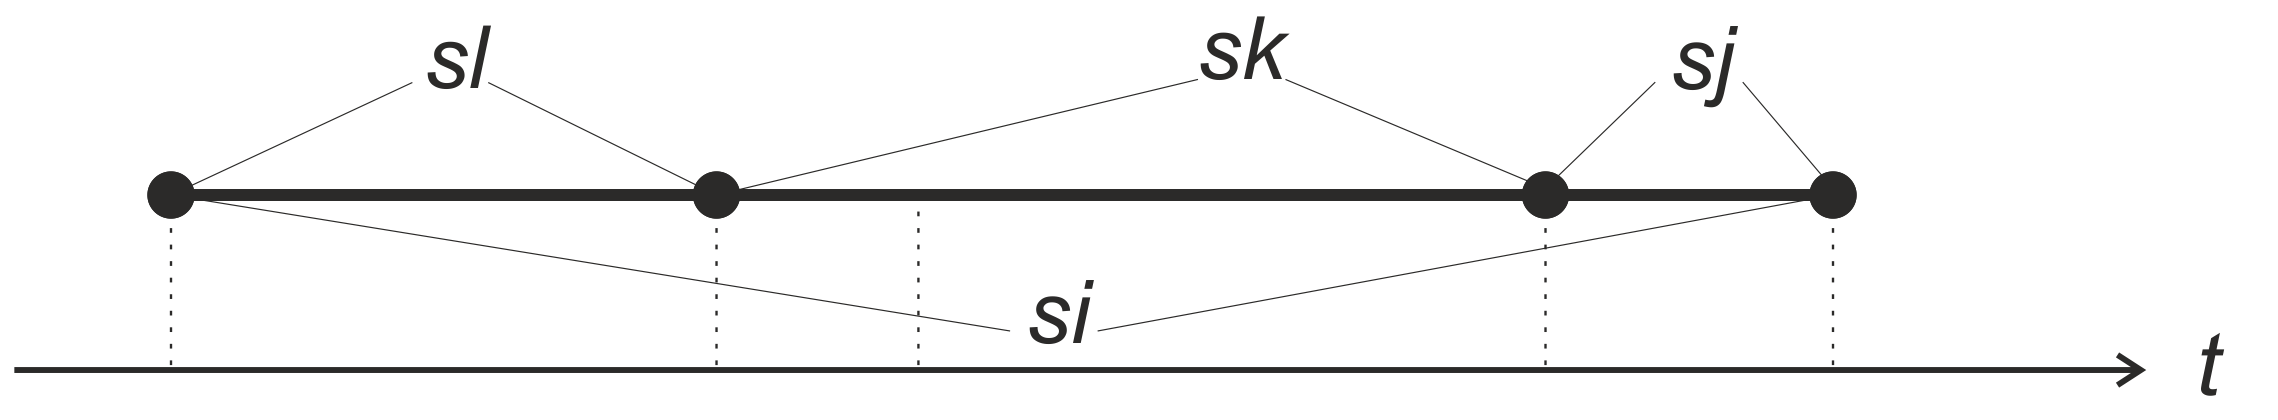
\includegraphics[width=1\linewidth]{figures/sd_temp_entities/img_temporal_decomposition.png}
}}

\scnheader{темпоральная смежность*}
\scnidtf{строгая темпоральная последовательность (без темпорального промежутка)*}
\scnidtf{темпоральная последовательность без промежутка*}
\scnrelfrom{типичная семантическая окрестность}{
\scnfilescg{figures/sd_temp_entities/temporal_adjacency.png}}
\scnrelfrom{иллюстрация}{
\scnfileimage{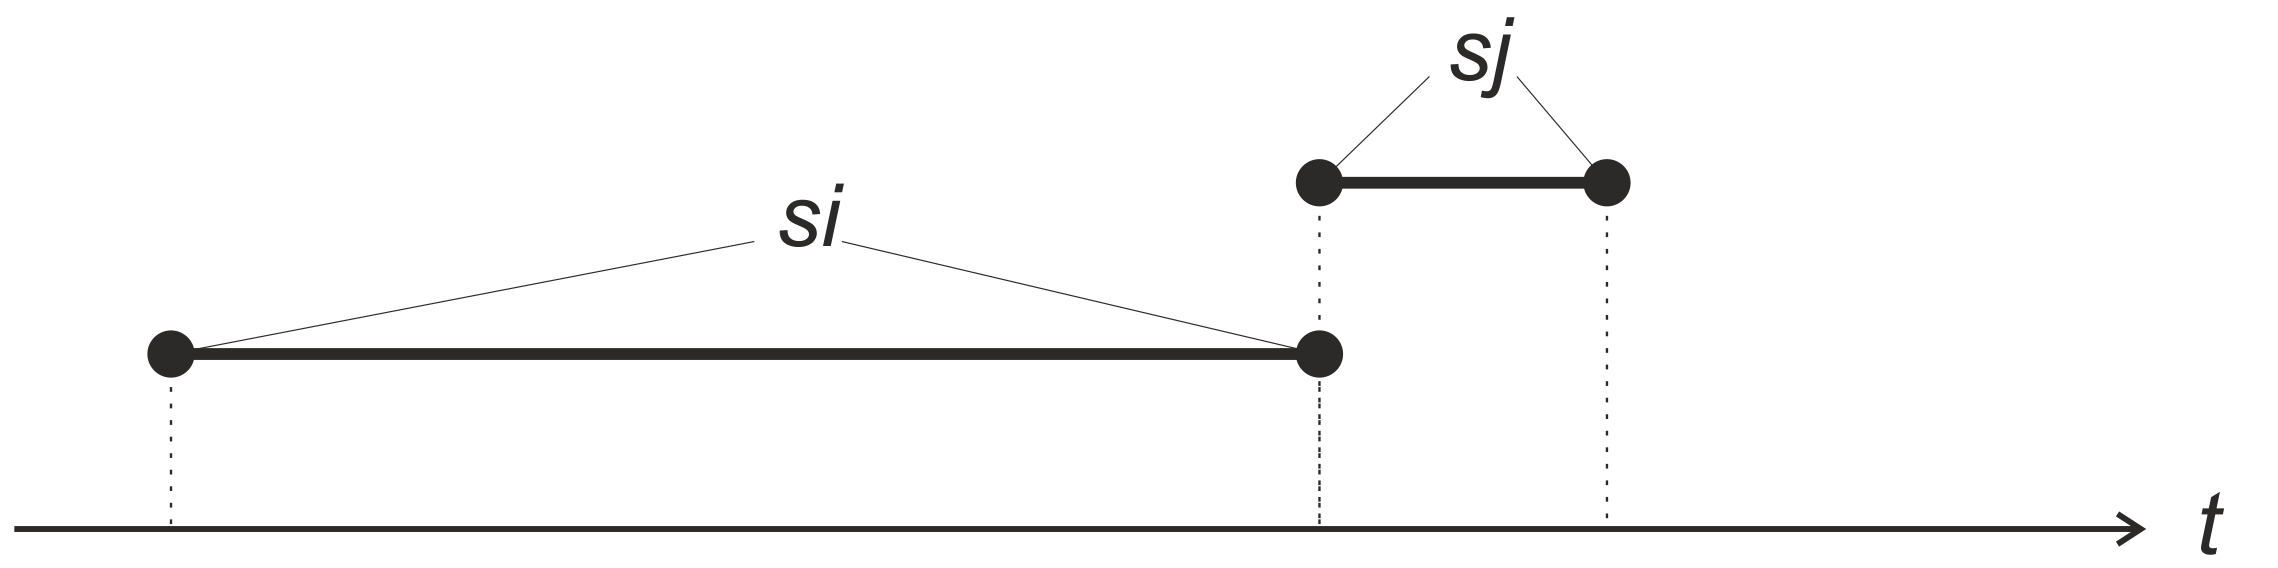
\includegraphics[width=1\linewidth]{figures/sd_temp_entities/img_temporal_adjacency.png}
}}

\scnheader{темпоральная последовательность с промежутком*}
\scnrelfrom{типичная семантическая окрестность}{
\scnfilescg{figures/sd_temp_entities/temporal_sequence_with_intermediate.png}}
\scnrelfrom{иллюстрация}{
\scnfileimage{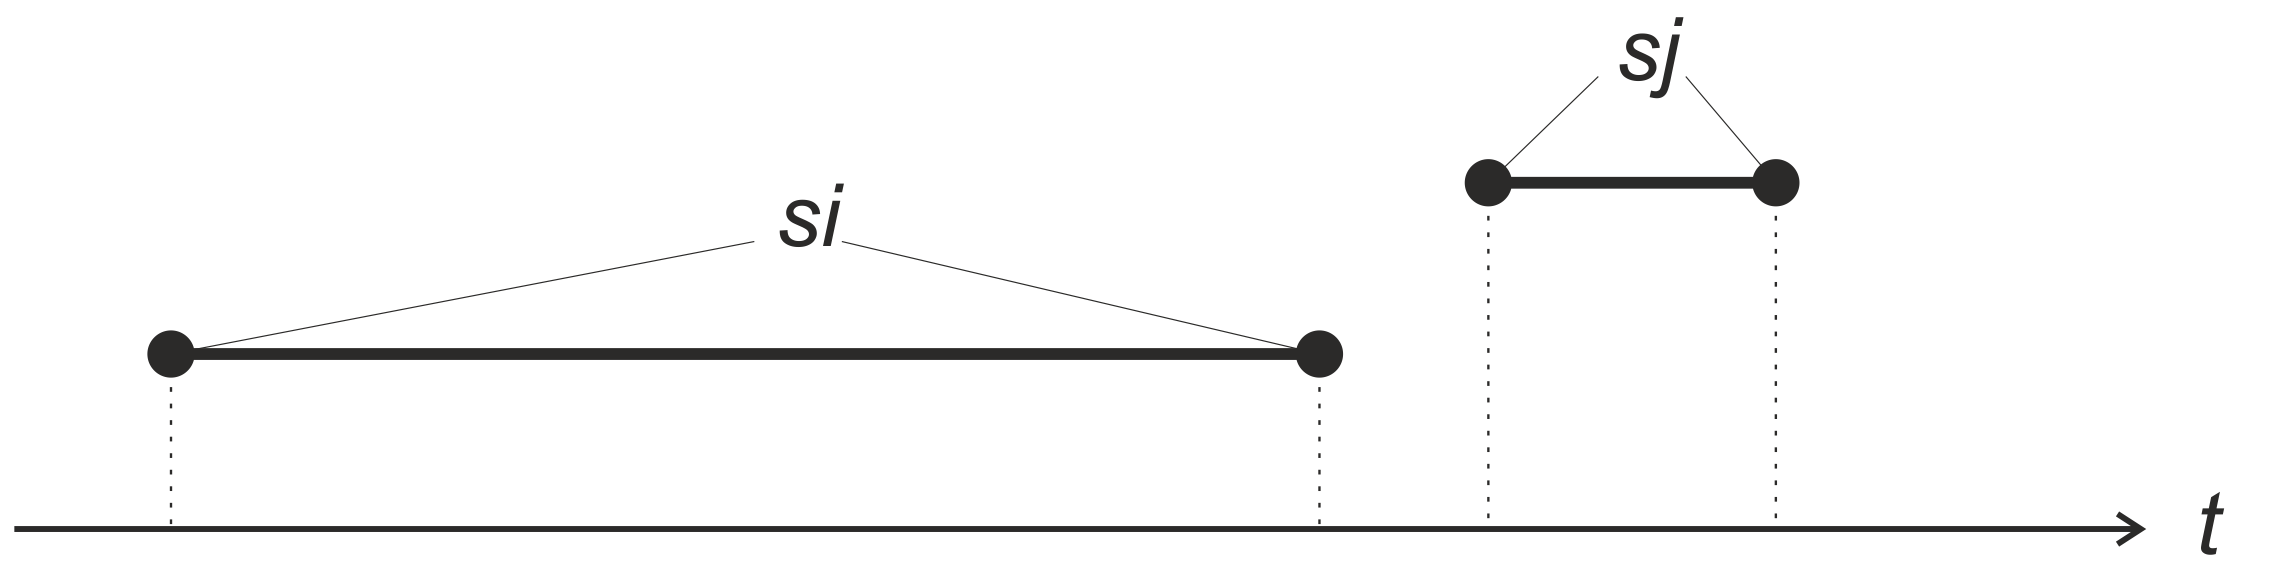
\includegraphics[width=1\linewidth]{figures/sd_temp_entities/img_temporal_sequence_with_intermediate.png}}}

\scnheader{темпоральная последовательность с пересечением*}
\scnrelfrom{типичная семантическая окрестность}{
\scnfilescg{figures/sd_temp_entities/temporal_sequence_with_intersection.png}
}
\scnrelfrom{иллюстрация}{
\scnfileimage{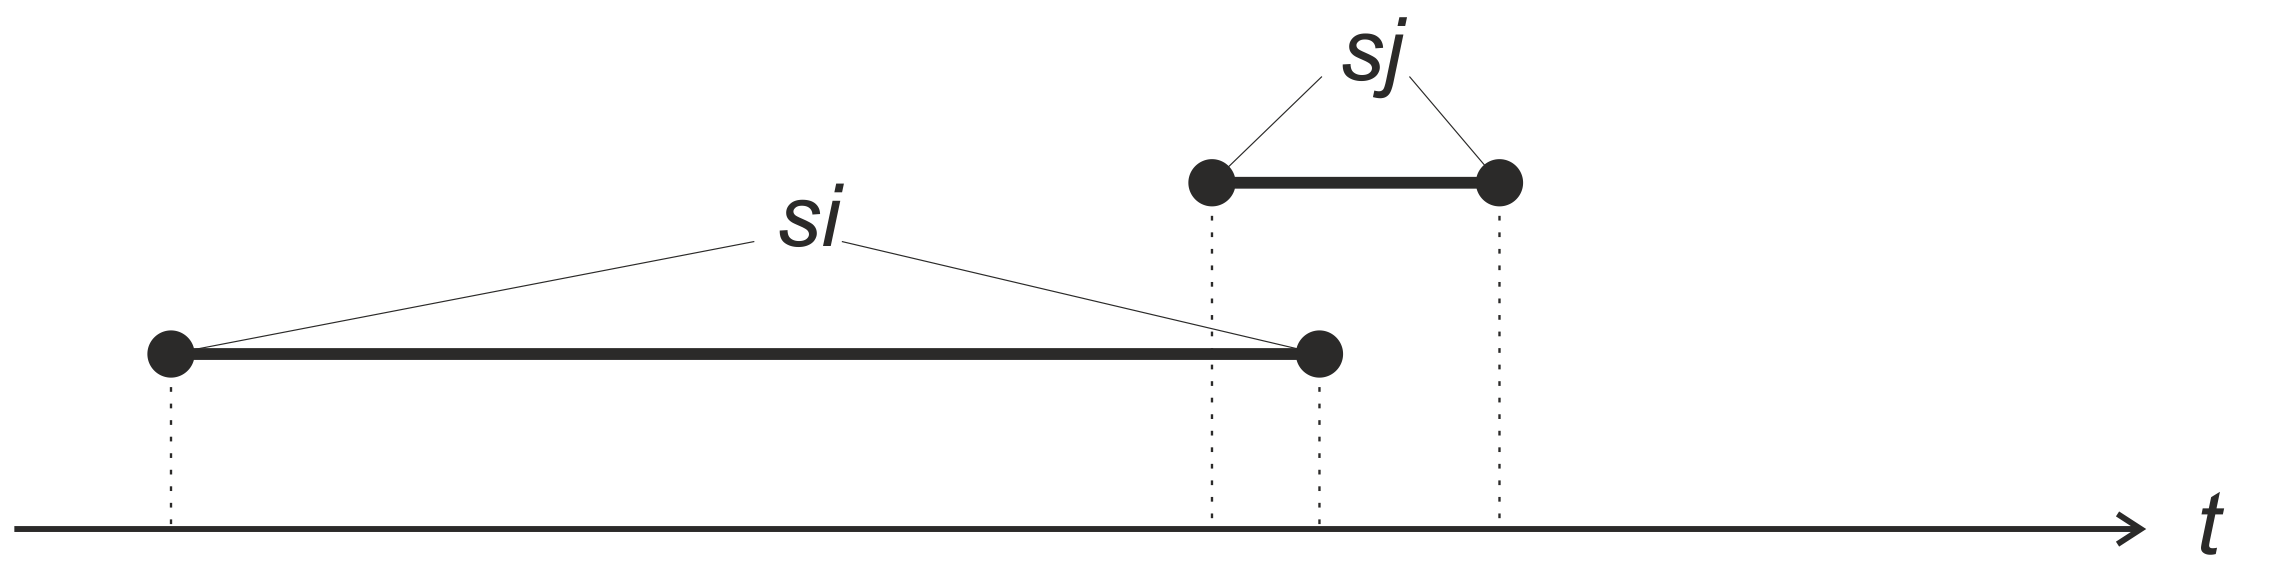
\includegraphics[width=1\linewidth]{figures/sd_temp_entities/img_temporal_cross_sequence.png}
}}

\scnheader{начало}
\scnidtf{класс одновременно начавшихся сущностей}
\scniselement{параметр}
\scnexplanation{Каждый элемент множества \textbf{начало} представляет собой класс \textit{временных сущностей}, у которых совпадает момент начала их существования. Конкретное значение данного \textit{параметра} может быть как \textit{точной величиной}, так и \textit{неточной величиной} или \textit{интервальной величиной}.}
\scnrelfrom{типичная семантическая окрестность}{
\scnfilescg{figures/sd_temp_entities/start.png}}
\scncomment{В данном примере \textbf{\textbf{\textit{ki}}} обозначает класс сущностей, начавших свое существование 19 февраля 2015 года по григорианскому календарю. Конкретные примеры таких сущностей – \textbf{\textit{bi}} и \textbf{\textit{bj}}. \textbf{\textit{ti}} обозначает временную точку григорианского календаря, соответствующую 19 февраля 2015 года.}

\scnheader{завершение}
\scnidtf{конец}
\scnidtf{класс одновременно завершившихся сущностей}
\scniselement{параметр}
\scnexplanation{Каждый элемент множества \textbf{\textit{завершение}} представляет собой класс \textit{временных сущностей}, у которых совпадает конечный момент их существования (момент завершения существования). Конкретное значение данного \textit{параметра} может быть как \textit{точной величиной}, так и \textit{неточной величиной} или \textit{интервальной величиной}.}
\scnrelfrom{типичная семантическая окрестность}{
\scnfilescg{figures/sd_temp_entities/completion.png}}
\scncomment{В данном примере \textbf{\textit{ki}} обозначает класс сущностей, завершивших свое существование 21 февраля 2015 года по григорианскому календарю. Конкретные примеры таких сущностей – \textbf{\textit{bi}} и \textbf{\textit{bj}}. \textbf{\textit{ti}} обозначает временную точку григорианского календаря, соответствующую 21 февраля 2015 года.}

\scnheader{длительность}
\scnidtf{класс временных сущностей, имеющих одинаковую длительность}
\scniselement{параметр}
\scnhaselement{тысячелетие}
\scnhaselement{век}
\scnhaselement{год}
\scnhaselement{месяц}
\scnhaselement{день}
\scnhaselement{час}
\scnhaselement{минута}
\scnhaselement{секунда}
\scnexplanation{Каждый элемент множества \textbf{\textit{длительность}} представляет собой класс \textit{временных сущностей}, у которых совпадает длительность их существования. Конкретное значение данного \textit{параметра} может быть как \textit{точной величиной}, так и \textit{неточной величиной} или \textit{интервальной величиной}.}
\scnrelfrom{типичная семантическая окрестность}{
\scnfilescg{figures/sd_temp_entities/duration.png}}
\scncomment{В данном примере \textbf{\textit{ki}} обозначает класс сущностей, существовавших в течение 2 месяцев. Конкретный пример такой сущности – \textbf{\textit{bi}}.}

\scnheader{тысячелетие}

\scnheader{век}

\scnheader{год}

\scnheader{месяц}

\scnheader{сутки}

\scnheader{час}

\scnheader{минута}

\scnheader{секунда}

\scnheader{номер тысячелетия\scnrolesign}
\scnheader{номер века\scnrolesign}
\scnheader{номер года\scnrolesign}
\scnheader{номер месяца в году\scnrolesign}
\scnheader{номер суток в месяце\scnrolesign}
\scnheader{номер часа в дне\scnrolesign}
\scnheader{номер минуты в часе\scnrolesign}
\scnheader{номер секунды в минуте\scnrolesign}

\scnendstruct

\end{SCn}